\part{Capítulo doce}

%----------------------------------------------------------------------------------------
%	CHAPTER 12
%----------------------------------------------------------------------------------------
\graphicspath{ {12_Capitulo/img/ejemplos/}, {W_Varios/2_Portada_capitulos/} }

\chapterimage{ima2} % Chapter heading image


\chapter{Relación Beneficio/Costo}

\section{Mapa Mental}

\begin{center}
   \includegraphics[height=6cm]{Mapa Mental 12.1.pdf}
\end{center} 


\section{Formulas de los capítulos}

\begin{spacing}{1.5}
	\begin{center}
		\begin{tabular}{ |p{4cm}|p{7cm}| p{4cm}|}
			\hline
			\rowcolor{orange!50}
			\begin{center}\textbf{Fórmula} \end{center} & \begin{center} \textbf{Nombre}\end{center}             & \begin{center} \textbf{Excel} \end{center}             \\ \hline
			
			B/C = $\frac{VPN}{VPC}$   & Relación Beneficio/Costo              & B/C = beneficio / (costo + Inversión) \\ \hline
			
			VP = $\frac{R}{i}$        & Valor Presente Serie Perpetua Vencida &                                       \\ \hline
		\end{tabular}
	\end{center}
\end{spacing}

\section{Introducción}
La relación Beneficio/Costo (B/C), consiste en poner en valor presente los beneficios netos y dividirlos por el valor presente de todos los costos del proyecto. La tasa que se utilice para poner en valor presente, tanto los beneficios como los costos, depende de quien lleve a cabo el proyecto, si el proyecto es particular se utiliza la tasa del inversionista, pero si éste es estatal se puede usar la tasa de interés social (que es más baja lo cual hace que la aceptación sea mas probable), de acuerdo a lo anterior podemos plantear la siguiente ecuación:

\begin{equation}
	B/C = \frac{Valor Presente de Ingresos(VP)}{Valor Presente de Costos(VPC)} \hspace{35pt} \textit{Relación Beneficio Costo (B/C)}
\end{equation}

La Relación B/C puede por tanto tomar tres valores:

% Incluir grafica 12_1
\begin{center}
	\includegraphics[height=3.0cm]{E12_1}
\end{center}

Si B/C < 1 significa que los ingresos son menores que los costos, por tanto el proyecto no es aconsejable.
\\
Si B/C = 1 significa que un valor presente, los ingresos son iguales a los egresos, en éste caso, lo único que se alcanza a ganar es la tasa del inversionista, por lo tanto es indiferente realizar el proyecto o continuar con la inversión que normalmente hace el inversionista.
\\
Si B/C  > 1 significa que en valor presente, los ingresos son mayores que los egresos, por lo tanto se aconseja realizar el proyecto.
\\
Las entidades crediticias tales como: Banco Mundial, Banco Internacional de Desarrollo, Fondo Monetario Internacional, etc., acostumbran a evaluar sus proyectos de inversión mediante la Relación B/C y adicionalmente con otro índice que generalmente es el VPN(Valor Presente Neto). Por esto es de gran importancia que cualquier proyecto que debido a su tamaño necesite financiación internacional sea evaluado con la Relación B/C.

\section{Beneficios, déficit , ventajas y desventajas en los proyectos}

Por lo general, los grandes proyectos son propiedad del estado y producen un beneficio para la sociedad,pero a su vez también pueden causar perdidas a las que llamaremos déficit  o desventajas y los costos del proyecto son los dineros invertidos por el estado.
\\
Es importante aclarar que el beneficio neto se representara con la letra B, es decir el beneficio menos el déficit. Para facilitar la identificación de las cantidades que corresponden a beneficios, déficit  y costos, podemos asumir, que en proyectos estatales, el que recibe los beneficios es la sociedad, el que recibe los déficit  también es la sociedad y el que hace los gastos es el estado. En proyectos particulares, el dueño del proyecto es quién recibe los beneficios, los déficit  y a su vez es el que hace sus gastos.
\\

\textbf{Ejemplo 1}\\
Para realizar un proyecto se necesita realizar una inversión inicial de 80.000 COP y otra inversión de
45.000 COP al final del primer mes, en los meses 2 y 3 los ingresos son equivalentes a los egresos;
pero a partir del mes 4, se producen ingresos así: Mes cuatro 30.000 COP, mes cinco 50.000 COP, mes
seis 60.000 COP. Determinar si el proyecto lo pueden realizar los inversionistas A o B mencionados
anteriormente.\\


%%%%%%%%%%%%%%%%%%% EJERCICIO 1 %%%%%%

%\newpage %USAR SOLO SI EL SOLUCION QUEDA SOLO Y ES NECESARIO BAJARLO A LA SIGUIENTE PAGINA
\textbf{Solución.}\\
%La tabla ira centrada
\begin{center}
	\renewcommand{\arraystretch}{1.5}% Margenes de las celdas
	%Creacion de la cuadricula de 3 columnas \end{flushleft}
	\begin{longtable}[H]{|C{0.3\linewidth}|C{0.3\linewidth}|C{0.3\linewidth}|}
		%Creamos una linea horizontal
		\hline
         %%%%% INICIO FLUJO DE CAJA
		\rowcolor[HTML]{FFB183}
		\multicolumn{3}{|c|}{\cellcolor[HTML]{FFB183}\textbf{1. Asignación periodo focal}}   \\ \hline
		\multicolumn{3}{|c|} {$pf = 0 pmv$} \\ \hline
		%%%%%%%%%% FIN TITULO
		%%%%%%%%%% INICIO TITULO
		%Lo que se hace aqui es mezclar las 3 columnas en una sola
		\multicolumn{3}{|c|}{\cellcolor[HTML]{FFB183}\textbf{2. Declaración de variables}}   \\ \hline
		%%%%%%%%%% FIN TITULO
		%%%%%%%%%% INICIO DE MATEMATICAS
		%Cada & hace referencia al paso de la siguiente columna
		$n_{0} = 0 pmv$   & $n_{1} = 1 pmv$ & $n_{2} =  4 pmv$\\
		$n_{3} = 5 pmv$ & $n_{4} = 6 pmv$ & \\ \hline
		\multicolumn{3}{|c|}{$i_{a} = TIO_{a} = 3\% \equiv 0.03 pmv$} \\
		\multicolumn{3}{|c|}{$i_{b} = TIO_{b} = 2\% \equiv 0.02 pmv$} \\ \hline
		%%%%%%%%%% FIN DE MATEMATICAS
		%%%%% FIN DECLARACION DE VARIABLES


		%%%%% INICIO FLUJO DE CAJA
		\rowcolor[HTML]{FFB183}
		\multicolumn{3}{|c|}{\cellcolor[HTML]{FFB183}\textbf{3. Diagrama de flujo de caja}} \\ \hline
		%Mezclamos 3 columnas y ponermos el dibujo
		%%%%%%%%%%%%% INSERCION DE LA IMAGEN
		%Deberan descargar las imagenes respectivas del drive y pegarlas en la carpeta
		%n_capitulo/img/ejemplos/1/capitulo1ejemplo1.pdf  (el /1/ es el numero del ejemplo)
		\multicolumn{3}{|c|}{ 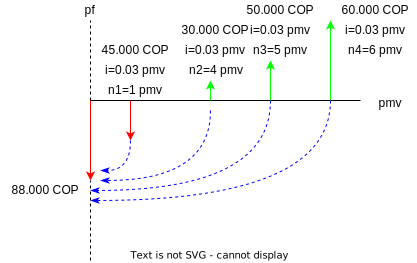
\includegraphics[trim=-5 -5 -5 -5 , scale=1.0,width=300px, height=250px]{9_Capitulo/ejemplos/1/Capitulo9Ejercicio1.pdf} }   \\ \hline
		%%%%%%%%%%%%% FIN INSERCION DE IMAGEN
		%%%%%FIN FLUJO DE CAJA



		%%%%% INICIO DECLARACION FORMULAS
		%%%%%%%%%%% INICIO TITULO
		\rowcolor[HTML]{FFB183}
		\multicolumn{3}{|c|}{\cellcolor[HTML]{FFB183}\textbf{4. Declaración de fórmulas}}    \\ \hline
		%%%%%%%%%%% FIN TITULO
		%%%%%%%%%%% INICIO MATEMATICAS
		\multicolumn{3}{|c|}{$\sum F_{n}(1+i)^{-n} $\hspace{0.3cm} \textit{Valor presente neto}} \\ \hline
		%%%%%%%%%% FIN MATEMATICAS
		%%%%%% INICIO DESARROLLO MATEMATICO
		\rowcolor[HTML]{FFB183}
		%%%%%%%%%%INICIO TITULO
		\multicolumn{3}{|c|}{\cellcolor[HTML]{FFB183}\textbf{5. Desarrollo matemático}}       \\ \hline
		%%%%%%%%%% FIN TITULO
		%%%%%%%%%% INICIO MATEMATICAS
		\multicolumn{3}{|c|}{$VPN_{a} = -80000 - 45000(1+0.03)^{-1} + 30000(1+0.03)^{-4} + 50000(1+0.03)^{-5} + 60000(1+0.03)^{-6}$} \\
		\multicolumn{3}{|c|}{$VPN_{a} = -3655$} \\
		\multicolumn{3}{|c|}{$VPN_{b} = -80000 - 45000(1+0.02)^{-1} + 30000(1+0.02)^{-4} + 50000(1+0.02)^{-5} + 60000(1+0.02)^{-6}$} \\
		\multicolumn{3}{|c|}{$VPN_{b} = 216254$} \\ \hline

		%%%%%%%%%% FIN MATEMATICAS
		%%%%%% FIN DESARROLLO MATEMATICO
		%%%%%% INICIO RESPUESTA
		\rowcolor[HTML]{FFB183}
		%%%%%%%%%%INICIO TITULO
		\multicolumn{3}{|c|}{\cellcolor[HTML]{FFB183}\textbf{6. Respuesta}}   \\ \hline
		%%%%%%%%%% FIN TITULO
		%%%%%%%%%% INICIO RESPUESTA MATEMATICA
		\multicolumn{3}{|c|}{Para B el $VPN > 0$, significa que puede realizar el proyecto en pesos de hoy,} \\ 
		\multicolumn{3}{|c|}{además de ganarse el 2\%, obtiene una ganancia de 2.162,54 COP.}  \\ \hline
		%%%%%%%%%% FIN MATEMATICAS
		%%%%%% FIN RESPUESTA
	\end{longtable}
	%Se crean dos lineas en blanco para que no quede el siguiente texto tan pegado
	%\newline \newline %USARLO SI CREES QUE ES NECESARIO
\end{center}
%%%%%%%%%%%%%%%%%%%%%%%%%%FIN EJERCICIO 1 %%%%%%%%%%%%%%%%%%%%%%%%%%%



\section{Relación B/C Y VPN}
Ocasionalmente se puede presentar una inconsistencia cuando se evalúan alternativas con la Relación B/C y con el VPN, en tales circunstancias el error debe estar en la Relación B/C causado por un incorrecto cálculo de los beneficios, entonces, se debe analizar lo que pasa con el exceso de inversión, es decir, que debe aplicarse el método incremental en la Relación B/C.
\\

\textbf{Ejemplo 2}\\
Se invierten 200{.}000 COP en un depósito a término fijo de 6 meses en un banco que paga el 28\% namv. Determinar el monto de la entrega al vencimiento.\\

%%%%%%%%%%%%%%%%%%% EJERCICIO 1 %%%%%%

%\newpage %USAR SOLO SI EL SOLUCIÓN QUEDA SOLO Y ES NECESARIO BAJARLO A LA SIGUIENTE PAGINA
\textbf{Solución.}
%La tabla ira centrada
\begin{center}
  \renewcommand{\arraystretch}{1.5}% Margenes de las celdas
  %Creación de la cuadricula de 3 columnas \end{flushleft}
  \begin{longtable}[H]{|C{0.3\linewidth}|C{0.3\linewidth}|C{0.3\linewidth}|}
    %Creamos una linea horizontal
    \hline
    %Definimos el color de la primera fila
    \rowcolor[HTML]{FFB183}
    %%%%% INICIO ASIGNACIÓN FECHA FOCAL %%%%%%%
    %%%%%%%%%% INICIO TITULO
    %Lo que se hace aquí es mezclar las 3 columnas en una sola
    \multicolumn{3}{|c|}{\cellcolor[HTML]{FFB183}\textbf{1. Asignación período focal}}                                  \\ \hline
    %%%%%%%%%% FIN TITULO
    %%%%% INICIO DECLARACIÓN DE VARIABLES %%%%%%%
    \multicolumn{3}{|c|}{$pf = 6pmv$}                                                                                   \\ \hline
    %%%%%%%%%% INICIO TITULO
    %Lo que se hace aquí es mezclar las 3 columnas en una sola
    \multicolumn{3}{|c|}{\cellcolor[HTML]{FFB183}\textbf{2. Declaración de variables}}                                  \\ \hline
    %%%%%%%%%% FIN TITULO
    %%%%%%%%%% INICIO DE MATEMÁTICAS
    %Cada & hace referencia al paso de la siguiente columna
    $P =  200{.}000$ COP & $n = 6\textit{pmv} $ & $i= ?\% pmv$                                                           \\
    $j=28\%namv$         & $m=12pmv$            & $F = ? COP$                                                           
    \\\hline

    %%%%%%%%%% FIN DE MATEMÁTICAS
    %%%%% FIN DECLARACIÓN DE VARIABLES


    %%%%% INICIO FLUJO DE CAJA
    \rowcolor[HTML]{FFB183}
    \multicolumn{3}{|c|}{\cellcolor[HTML]{FFB183}\textbf{3. Diagrama de flujo de caja}}                                 \\ \hline
    %Mezclamos 3 columnas y pondremos el dibujo
    %%%%%%%%%%%%% INSERCIÓN DE LA IMAGEN
    %Deberán descargar las imágenes respectivas del drive y pegarlas en la carpeta
    %n_capitulo/img/ejemplos/1/capitulo1ejemplo1.pdf  (el /1/ es el numero del ejemplo)
    \multicolumn{3}{|c|}{ 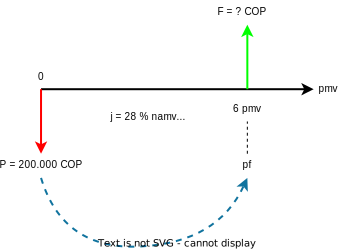
\includegraphics[trim=-5 -5 -5 -5 , scale=1]{2_Capitulo/ejemplos/2/Capitulo2Ejercicio2_v2.pdf} } \\ \hline
    %%%%%%%%%%%%% FIN INSERCIÓN DE IMAGEN
    %%%%%FIN FLUJO DE CAJA



    %%%%% INICIO DECLARACIÓN FORMULAS
    %%%%%%%%%%% INICIO TITULO
    \rowcolor[HTML]{FFB183}
    \multicolumn{3}{|c|}{\cellcolor[HTML]{FFB183}\textbf{4. Declaración de fórmulas}}                                   \\ \hline
    %%%%%%%%%%% FIN TITULO
    %%%%%%%%%%% INICIO MATEMÁTICAS
    \multicolumn{3}{|c|}{$F = P(1+i)^n \hspace{0.3cm} \textit{Valor futuro}$}                                           \\
    \multicolumn{3}{|c|}{$j=i\cdot m\hspace{0.3cm}\textit{Tasa periódica anualizada}$}
    \\ \hline
    %%%%%%%%%% FIN MATEMÁTICAS
    %%%%%% INICIO DESARROLLO MATEMÁTICO
    \rowcolor[HTML]{FFB183}
    %%%%%%%%%%INICIO TITULO
    \multicolumn{3}{|c|}{\cellcolor[HTML]{FFB183}\textbf{5. Desarrollo matemático}}                                     \\ \hline
    %%%%%%%%%% FIN TITULO
    %%%%%%%%%% INICIO MATEMÁTICAS
    \multicolumn{3}{|c|}{$0{.}28=i\cdot 12$}                                                                            \\
    \multicolumn{3}{|c|}{$i= \frac{0{.}28}{12} = 0{.}02333... \equiv 2{.}333\%pmv$}                                     \\
    \multicolumn{3}{|c|}{$0{.}28=i\cdot 12$}                                                                            \\
    \multicolumn{3}{|c|}{$F = 200{.}000 COP(1+0,2333)^6$}                                                       \\
    \multicolumn{3}{|c|}{$F = 229{.}685.04 COP$}
    \\ \hline


    %%%%%%%%%% FIN MATEMÁTICAS
    %%%%%% FIN DESARROLLO MATEMÁTICO
    %%%%%% INICIO RESPUESTA
    \rowcolor[HTML]{FFB183}
    %%%%%%%%%%INICIO TITULO
    \multicolumn{3}{|c|}{\cellcolor[HTML]{FFB183}\textbf{6. Respuesta}}                                                 \\ \hline
    %%%%%%%%%% FIN TITULO
    %%%%%%%%%% INICIO RESPUESTA MATEMÁTICA
    \multicolumn{3}{|c|}{$F = 229{.}685.04 COP$
    }                                                                                                                   \\ \hline
    %%%%%%%%%% FIN MATEMÁTICAS
    %%%%%% FIN RESPUESTA
  \end{longtable}
  %Se crean dos lineas en blanco para que no quede el siguiente texto tan pegado
  %\newline \newline %USARLO SI CREES QUE ES NECESARIO
\end{center}
%%%%%%%%%%%%%%%%%%%%%%%%%%FIN EJERCICIO 1 %%%%%%%%%%%%%%%%%%%%%%%%%%%



\section{Periodo de recuperación}
El Período de Recuperación, PR, es otro índice utilizado para medir la bondad de un proyecto, sin embargo este ha venido perdiendo popularidad dandole paso al VPN y a la TIR que son mucho más exactos. El PR es el tiempo que debe utilizarse para recuperar la inversión, sin tener en cuenta los intereses; Por ejemplo, si se invierten  COP 600.000 en un proyecto que produce  COP 200.000 anuales durante 8 años, entonces se necesitarán 3 años para recuperar la inversión inicial (3 x 200.000 = 600.000) y, de ahí en adelante, lo que se produzca se considera ganancia. Si el propietario del proyecto considera que 3 años es un tiempo razonable para recuperar la inversión, el proyecto será aceptado, pero si considera que no puede esperar tanto tiempo, el proyecto será rechazado.\\

Entre las fallas técnicas que presenta el PR está la de no tomar en cuenta el valor del dinero a través del tiempo y la de no tomar en cuenta el flujo de caja después de la recuperación de los dineros invertidos. En el siguiente ejemplo, se podrán observar estas fallas.\\

\textbf{Ejemplo 3}\\
Una fabrica produce actualmente en forma manual 1.000 unidades de un determinado artículo, para ello utiliza artesanos a los cuales les paga 8.400.000 COP al año y, es costumbre que cada año se les aumente el sueldo en aproximadamente un 20\%. El precio de venta de cada artículo es de 9.000 COP y se estima que este precio podrá ser aumentado todos los años en un 21\%. Ahora se ha presentado la oportunidad de adquirir una máquina a un costo de 10 millones COP con una vida útil de 5 años; un valor de salvamento de 2 millones COP la cual requiere de 2 técnicos para su operación, el sueldo anual de cada uno de los técnicos puede ser de 600.000 COP con aumentos anuales de sueldo del 20\% ¿Cuál de las dos alternativas es mejor suponiendo que la tasa del inversionista es del 30\%?\\


%%%%%%%%%%%%%%%%%%% EJERCICIO 3 %%%%%%

%\newpage %USAR SOLO SI EL SOLUCION QUEDA SOLO Y ES NECESARIO BAJARLO A LA SIGUIENTE PAGINA
\textbf{Solución.}\\
%La tabla ira centrada
\begin{center}
	\renewcommand{\arraystretch}{1.5}% Margenes de las celdas
	%Creacion de la cuadricula de 3 columnas \end{flushleft}
	\begin{longtable}[H]{|C{0.3\linewidth}|C{0.3\linewidth}|C{0.3\linewidth}|}
		%Creamos una linea horizontal
		\hline
        %%%%% INICIO FLUJO DE CAJA
		\rowcolor[HTML]{FFB183}
		\multicolumn{3}{|c|}{\cellcolor[HTML]{FFB183}\textbf{1. Asignación periodo focal}}   \\ \hline
		\multicolumn{3}{|c|} {$pf = 0 pav$} \\ \hline
		%%%%%%%%%% FIN TITULO
		%%%%%%%%%% INICIO TITULO
		%Lo que se hace aqui es mezclar las 3 columnas en una sola
		\multicolumn{3}{|c|}{\cellcolor[HTML]{FFB183}\textbf{2. Declaración de variables}}   \\ \hline
		%%%%%%%%%% FIN TITULO
		%%%%%%%%%% INICIO DE MATEMATICAS
		%Cada & hace referencia al paso de la siguiente columna
		$R_{1} = 9.000.000 $ COP   & $R_{2} = 8.400.000$ COP  & $i=0.3pav$\\ 
		$g_{1} =  0.21 pav $ & $g_{2}=  0.2 pav $ & $n=5pav$ \\ \hline
		%%%%%%%%%% FIN DE MATEMATICAS
		%%%%% FIN DECLARACION DE VARIABLES

  		%%%%% INICIO DECLARACION FORMULAS
  
		%%%%%%%%%%% INICIO TITULO
		\rowcolor[HTML]{FFB183}
		\multicolumn{3}{|c|}{\cellcolor[HTML]{FFB183}\textbf{3. Diagrama de flujo de caja}} \\ \hline
		%Mezclamos 3 columnas y ponermos el dibujo
		%%%%%%%%%%%%% INSERCION DE LA IMAGEN
		%Deberan descargar las imagenes respectivas del drive y pegarlas en la carpeta
		%n_capitulo/img/ejemplos/1/capitulo1ejemplo1.pdf  (el /1/ es el numero del ejemplo)
		\multicolumn{3}{|c|}{ \includegraphics[trim=-5 -5 -5 -5 , scale=1, width=300px, height=250px]{9_Capitulo/ejemplos/3/Capitulo9Ejercicio3.pdf} }   \\ \hline
		%%%%%%%%%%%%% FIN INSERCION DE IMAGEN
		%%%%%FIN FLUJO DE CAJA



		%%%%% INICIO DECLARACION FORMULAS
		%%%%%%%%%%% INICIO TITULO
		\rowcolor[HTML]{FFB183}
		\multicolumn{3}{|c|}{\cellcolor[HTML]{FFB183}\textbf{4. Declaración de fórmulas}}    \\ \hline
		%%%%%%%%%%% FIN TITULO
		%%%%%%%%%%% INICIO MATEMATICAS
		\multicolumn{3}{|c|}{$\sum F_{n}(1+i)^{-n} $\hspace{0.3cm} \textit{Valor presente neto}} \\ \hline
		%%%%%%%%%% FIN MATEMATICAS
		%%%%%% INICIO DESARROLLO MATEMATICO
		\rowcolor[HTML]{FFB183}
		%%%%%%%%%%INICIO TITULO
		\multicolumn{3}{|c|}{\cellcolor[HTML]{FFB183}\textbf{5. Desarrollo matemático}}       \\ \hline
		%%%%%%%%%% FIN TITULO
		%%%%%%%%%% INICIO MATEMATICAS
		\multicolumn{3}{|c|}{$VPN_{A} = \frac{9[(1+0.21)^{5}(1+0.3)^{-5} -1]}{0.21-0.3} - \frac{8.4[(1+0.2)^{5}(1+0.3^{-5} -1)]}{0.2-0.3}$} \\
		\multicolumn{3}{|c|}{$VPN_{A} = 2.437.836 $ COP} \\
		\multicolumn{3}{|c|}{$VPN_{B} = \frac{9[(1+0.21)^{5}(1+0.3)^{-5} -1]}{0.21-0.3} + 2(1.3)^{-5} - \frac{1.2[(1+0.2)^{5}(1+0.3^{-5} -1)]}{0.2-0.3}$} \\
		\multicolumn{3}{|c|}{$VPN_{B} = 16.723.756 $ COP} \\ \hline

		%%%%%%%%%% FIN MATEMATICAS
		%%%%%% FIN DESARROLLO MATEMATICO
		%%%%%% INICIO RESPUESTA
		\rowcolor[HTML]{FFB183}
		%%%%%%%%%%INICIO TITULO
		\multicolumn{3}{|c|}{\cellcolor[HTML]{FFB183}\textbf{6. Respuesta}}   \\ \hline
		%%%%%%%%%% FIN TITULO
		%%%%%%%%%% INICIO RESPUESTA MATEMATICA
		\multicolumn{3}{|c|}{La decisión correcta es comprar la máquina.}  \\ \hline
		%%%%%%%%%% FIN MATEMATICAS
		%%%%%% FIN RESPUESTA
	\end{longtable}
	%Se crean dos lineas en blanco para que no quede el siguiente texto tan pegado
	%\newline \newline %USARLO SI CREES QUE ES NECESARIO
\end{center}
%%%%%%%%%%%%%%%%%%%%%%%%%%FIN EJERCICIO 3 %%%%%%%%%%%%%%%%%%%%%%%%%%%

